% --------------------------------------------------------------
% This is all preamble stuff that you don't have to worry about.
% Head down to where it says "Start here"
% --------------------------------------------------------------
 
\documentclass[12pt]{article}
 
\usepackage[margin=1in]{geometry} 
\usepackage{amsmath,amsthm,amssymb}
\usepackage{gensymb}
\usepackage{graphicx}
 \usepackage{tikz,pgfplots}
\usepackage{float}
\usepackage{tikz}
\usepackage{enumitem}
\usetikzlibrary{calc}

\newcommand{\N}{\mathbb{N}}
\newcommand{\Z}{\mathbb{Z}}

\newcommand{\slantedgrid}[4]{%
   \pgfmathtruncatemacro{\result}{#1+#3}
   \foreach \x in {#1,...,\result} \draw (\x,#2) -- ++(#4,#4);%
   \pgfmathtruncatemacro{\result}{#2+#4}
   \foreach \y in {#2,...,\result} \draw (#1+\y-#2,\y) -- ++(#3,0);%
 }
 
\newenvironment{theorem}[2][Theorem]{\begin{trivlist}
\item[\hskip \labelsep {\bfseries #1}\hskip \labelsep {\bfseries #2.}]}{\end{trivlist}}
\newenvironment{lemma}[2][Lemma]{\begin{trivlist}
\item[\hskip \labelsep {\bfseries #1}\hskip \labelsep {\bfseries #2.}]}{\end{trivlist}}
\newenvironment{exercise}[2][Exercise]{\begin{trivlist}
\item[\hskip \labelsep {\bfseries #1}\hskip \labelsep {\bfseries #2.}]}{\end{trivlist}}
\newenvironment{problem}[2][Problem]{\begin{trivlist}
\item[\hskip \labelsep {\bfseries #1}\hskip \labelsep {\bfseries #2.}]}{\end{trivlist}}
\newenvironment{question}[2][Question]{\begin{trivlist}
\item[\hskip \labelsep {\bfseries #1}\hskip \labelsep {\bfseries #2.}]}{\end{trivlist}}
\newenvironment{corollary}[2][Corollary]{\begin{trivlist}
\item[\hskip \labelsep {\bfseries #1}\hskip \labelsep {\bfseries #2.}]}{\end{trivlist}}
 
\begin{document}
\providecommand{\e}[1]{\ensuremath{\times 10^{#1}}}
% --------------------------------------------------------------
%                         Start here
% --------------------------------------------------------------
 
\title{HW 3}%replace X with the appropriate number
\author{Levon Dovlatyan, SI: 24451582\\ %replace with your name
E45} %if necessary, replace with your course title
 
\maketitle
 
\begin{problem}{3.70}
The diffraction peaks labeled in Figure 3.33 correspond to the reflection rules for an FCC metal (h, k, l unmixed, as shown in Table 3.4). What would be the hkl indices for the three lowest diffraction-angle peaks for a bcc metal?
\end{problem}
 
The rule for bcc metals state that $h + k + l =$ even number. Also the indices start from the lowest possible combination and work up. Using these simple rules we can find the first 3 peaks.

\begin{figure}[H]
\centering
\begin{tabular}{c | c | c}
Peak & hkl indices & proof of even number \\ \hline
1 & (110) & $1+1+0=2$ \\ \hline
2 & (200) & $2+0+0=2$ \\ \hline
3 & (211) & $2+1+1=4$
\end{tabular}
\end{figure}

\begin{problem}{3.80}
Calculate the first six diffraction peak positions for MgO powder using Cu$\text{K}_{\alpha}$ radiation.  (This ceramic structure based on the fcc lattice shares the reflection rules of the fcc metals).
\end{problem}

The edge length $a$ of a fcc bravais lattice with two ions is $a = 2(r_{\text{anion}} + r_{\text{cation}})$. So the edge length for MgO is $a = 0.420$nm and $\lambda_{\text{CuK}_{\alpha}} = 0.1542$nm. Using this we can solve the Bragg's equation for the simple case of n = 1,

\begin{equation}
\theta = \arcsin{\frac{\lambda}{2d}}
\end{equation}
\begin{equation}
d = \frac{a}{\sqrt{h^2 + k^2 + l^2}}
\end{equation}

\begin{figure}[H]
\centering
\begin{tabular}{c | c | c | c}
Peak & hkl indices & $d_{hkl}$ (nm) & $2\theta$ (degrees) \\ \hline
1 & (111) & 0.242 & 37.1 \\ \hline
2 & (200) & 0.210 & 43.1 \\ \hline
3 & (220) & 0.148 & 62.6 \\ \hline
4 & (311) & 0.127 & 75.0 \\ \hline
5 & (222) & 0.121 & 79.0 \\ \hline
6 & (400) & 0.105 & 94.5 \\ 
\end{tabular}
\end{figure}

\begin{problem}{4.19}
Calculate the density of Schottky pairs (in $m^{-3}$) in MgO if the fraction of vacant lattice sites is $5\e{-6}$.  (The density of MgO is 3.60 Mg/$m^3$).
\end{problem}

\begin{align*}
\text{atom density} = \frac{\rho}{\text{atom mass}} = \frac{3.60 \e{6} g/m^3}{(24.31 + 16.00)g/(6.02\e{23}\text{atoms})} = 5.376 \e{28}\,\text{atoms}/m^3 \\ \\
\text{vacancy density} = 5\e{-6} \text{atoms}^{-1} \times 5.376\e{28} \text{atoms}*m^{-3} = 2.69 \e{23} m^{-3}
\end{align*}

\begin{problem}{4.21}
The energy necessary to generate a dislocation is proportional to the square of the length of the Burgers vector, $|b|^2$.  This relationship means that the most stable (lowest energy) dislocations have the minimum length, $|b|$.  For the bcc metal structure, calculate (relative to $E_{b=[111]}$) the dislocation energies for \textbf{(a)} $E_{b=[110]}$ and \textbf{(b)} $E_{b=[100]}$.
\end{problem}

Since $E \propto |b|^2$, we can compare ratios relative to $|b|_{[111]}$.  Also the edge length of a bcc is $a$ and the diagonal across the base is $\sqrt{2}a$. Note for a bcc, $a = 4R/\sqrt{3}$.\\*[0.5cm]
\textbf{(a)}
\begin{align*}
\frac{E_{b=[110]}}{E_{b=[111]}} = (\frac{|b_{[110]}|}{|b_{[111]|}})^2 = (\frac{\sqrt{2}a}{2R})^2 = (\frac{\sqrt{2}4R/\sqrt{3}}{2R})^2 = \frac{8}{3} = 2.67
\end{align*}
\textbf{(b)}
\begin{align*}
\frac{E_{b=[100]}}{E_{b=[111]}} = (\frac{|b_{[100]}|}{|b_{[111]|}})^2 = (\frac{a}{2R})^2 = (\frac{4R/\sqrt{3}}{2R})^2 = \frac{4}{3} = 1.33
\end{align*}

\begin{problem}{4.30}
As Figure 4.20 shows, noncrystalline metal has a range of space-filling polyhedra comprising its structure.  Similarly, the FCC structure can be represented by a repetitive polyhedra structure, which is an alternative to our usual unit cell configuration.  In other words, the fcc structure can be equally represented by a space-filling stacking of regular polyhedra (tetrahedra and octahedra in a ration of 2:1).  (a) Sketch a typical tetrahedron (four-sided figure) on a perspective sketch such as Figure 3.5(a).  (b)  Similarly, show a typical octahedron (eight-sided figure).  Note also Problem 3.60.)
\end{problem}
Drawn in latex using tikz package
\begin{figure}[H]
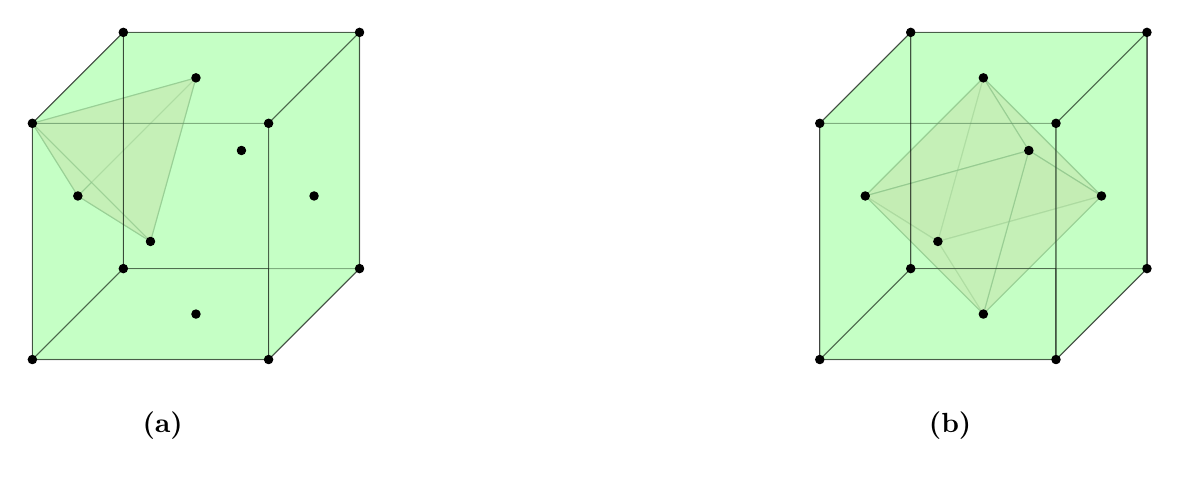
\begin{tikzpicture}[line join = round, line cap = round]
\pgfmathsetmacro{\factor}{1/sqrt(2)};
%\coordinate [label=right:A] (A) at (2,0,-2*\factor);
%\coordinate [label=left:B] (B) at (-2,0,-2*\factor);
%\coordinate [label=above:C] (C) at (0,2,2*\factor);
%\coordinate [label=below:D] (D) at (0,-2,2*\factor);

\coordinate [] (A) at (0,0,0);
\coordinate [] (B) at (0,0,3);
\coordinate [] (C) at (3,0,3);
\coordinate [] (D) at (3,0,0);
\coordinate [] (E) at (0,3,0);
\coordinate [] (F) at (0,3,3);
\coordinate [] (G) at (3,3,3);
\coordinate [] (H) at (3,3,0);

\coordinate [] (X) at (0,1.5,1.5);
\coordinate [] (Y) at (0,3,3);
\coordinate [] (Z) at (1.5,1.5,3);
\coordinate [] (L) at (1.5,3,1.5);

\draw[fill=red!30, opacity=.5] (X)--(Y)--(Z)--cycle;
\draw[fill=red!30, opacity=.5] (X)--(L)--(Z)--cycle;
\draw[fill=red!30, opacity=.5] (X)--(Y)--(L)--cycle;
\draw[fill=red!30, opacity=.5] (Z)--(Y)--(L)--cycle;

\draw[fill=green!30, opacity=.5] (A)--(B)--(C)--(D)--cycle;
\draw[fill=green!30, opacity=.5] (E)--(F)--(G)--(H)--cycle;
\draw[fill=green!30, opacity=.5] (F)--(B)--(C)--(G)--cycle;
\draw[fill=green!30, opacity=.5] (E)--(A)--(D)--(H)--cycle;
\draw[fill=green!30, opacity=.5] (C)--(D)--(H)--(G)--cycle;
\draw[fill=green!30, opacity=.5] (A)--(B)--(F)--(E)--cycle;

\draw[fill=black] (0,0,0) circle (0.15em);
\draw[fill=black] (0,0,3) circle (0.15em);
\draw[fill=black] (3,0,3) circle (0.15em);
\draw[fill=black] (3,0,0) circle (0.15em);
\draw[fill=black] (0,3,0) circle (0.15em);
\draw[fill=black] (0,3,3) circle (0.15em);
\draw[fill=black] (3,3,3) circle (0.15em);
\draw[fill=black] (3,3,0) circle (0.15em);

\draw[fill=black] (0,1.5,1.5) circle (0.15em);
\draw[fill=black] (3,1.5,1.5) circle (0.15em);
\draw[fill=black] (1.5,1.5,0) circle (0.15em);
\draw[fill=black] (1.5,1.5,3) circle (0.15em);
\draw[fill=black] (1.5,0,1.5) circle (0.15em);
\draw[fill=black] (1.5,3,1.5) circle (0.15em);

%%%%%%%%%%%%%%%%%%%%%%%%%%%%%%%%%%%%%%%%%%%%%%%%%%%%%%%%%%% part b

\coordinate [] (a) at (10,0,0);
\coordinate [] (b) at (10,0,3);
\coordinate [] (c) at (13,0,3);
\coordinate [] (d) at (13,0,0);
\coordinate [] (e) at (10,3,0);
\coordinate [] (f) at (10,3,3);
\coordinate [] (g) at (13,3,3);
\coordinate [] (h) at (13,3,0);

\coordinate [] (x) at (10,1.5,1.5);
\coordinate [] (y) at (11.5,1.5,3);
\coordinate [] (z) at (13,1.5,1.5);
\coordinate [] (l) at (11.5,1.5,0);
\coordinate [] (i) at (11.5,3,1.5);
\coordinate [] (j) at (11.5,0,1.5);

\draw[fill=red!30, opacity=.5] (x)--(y)--(z)--(l)--cycle; % plane
\draw[fill=red!30, opacity=.5] (i)--(x)--(y)--cycle; %top
\draw[fill=red!30, opacity=.5] (i)--(y)--(z)--cycle; %top
\draw[fill=red!30, opacity=.5] (i)--(z)--(l)--cycle; %top
\draw[fill=red!30, opacity=.5] (i)--(l)--(x)--cycle; %top
\draw[fill=red!30, opacity=.5] (j)--(x)--(y)--cycle; %bot
\draw[fill=red!30, opacity=.5] (j)--(y)--(z)--cycle; %bot
\draw[fill=red!30, opacity=.5] (j)--(z)--(l)--cycle; %bot
\draw[fill=red!30, opacity=.5] (j)--(l)--(x)--cycle; %bot

\draw[fill=green!30, opacity=.5] (a)--(b)--(c)--(d)--cycle;
\draw[fill=green!30, opacity=.5] (e)--(f)--(g)--(h)--cycle;
\draw[fill=green!30, opacity=.5] (f)--(b)--(c)--(g)--cycle;
\draw[fill=green!30, opacity=.5] (e)--(a)--(d)--(h)--cycle;
\draw[fill=green!30, opacity=.5] (c)--(d)--(h)--(g)--cycle;
\draw[fill=green!30, opacity=.5] (a)--(b)--(f)--(e)--cycle;

\draw[fill=black] (10,0,0) circle (0.15em);
\draw[fill=black] (10,0,3) circle (0.15em);
\draw[fill=black] (13,0,3) circle (0.15em);
\draw[fill=black] (13,0,0) circle (0.15em);
\draw[fill=black] (10,3,0) circle (0.15em);
\draw[fill=black] (10,3,3) circle (0.15em);
\draw[fill=black] (13,3,3) circle (0.15em);
\draw[fill=black] (13,3,0) circle (0.15em);

\draw[fill=black] (10,1.5,1.5) circle (0.15em);
\draw[fill=black] (13,1.5,1.5) circle (0.15em);
\draw[fill=black] (11.5,1.5,0) circle (0.15em);
\draw[fill=black] (11.5,1.5,3) circle (0.15em);
\draw[fill=black] (11.5,0,1.5) circle (0.15em);
\draw[fill=black] (11.5,3,1.5) circle (0.15em);

\node at (0.5,-2) {\textbf{(a)}};
\node at (10.5,-2) {\textbf{(b)}};


\end{tikzpicture}
\end{figure}


% --------------------------------------------------------------
%     You don't have to mess with anything below this line.
% --------------------------------------------------------------
 
\end{document}
